\documentclass[hidelinks,12pt]{article}
\usepackage[left=0.25cm,top=1cm,right=0.25cm,bottom=1cm]{geometry}
%\usepackage[landscape]{geometry}
\textwidth = 20cm
\hoffset = -1cm
\usepackage[utf8]{inputenc}
\usepackage[spanish,es-tabla]{babel}
\usepackage[autostyle,spanish=mexican]{csquotes}
\usepackage[tbtags]{amsmath}
\usepackage{nccmath}
\usepackage{amsthm}
\usepackage{amssymb}
\usepackage{mathrsfs}
\usepackage{graphicx}
\usepackage{subfig}
\usepackage{standalone}
\usepackage[outdir=./Imagenes/]{epstopdf}
\usepackage{siunitx}
\usepackage{physics}
\usepackage{color}
\usepackage{float}
\usepackage{hyperref}
\usepackage{multicol}
%\usepackage{milista}
\usepackage{anyfontsize}
\usepackage{anysize}
%\usepackage{enumerate}
\usepackage[shortlabels]{enumitem}
\usepackage{capt-of}
\usepackage{bm}
\usepackage{relsize}
\usepackage{placeins}
\usepackage{empheq}
\usepackage{cancel}
\usepackage{wrapfig}
\usepackage[flushleft]{threeparttable}
\usepackage{makecell}
\usepackage{fancyhdr}
\usepackage{tikz}
\usepackage{bigints}
\usepackage{scalerel}
\usepackage{pgfplots}
\usepackage{pdflscape}
\pgfplotsset{compat=1.16}
\spanishdecimal{.}
\renewcommand{\baselinestretch}{1.5} 
\renewcommand\labelenumii{\theenumi.{\arabic{enumii}})}
\newcommand{\ptilde}[1]{\ensuremath{{#1}^{\prime}}}
\newcommand{\stilde}[1]{\ensuremath{{#1}^{\prime \prime}}}
\newcommand{\ttilde}[1]{\ensuremath{{#1}^{\prime \prime \prime}}}
\newcommand{\ntilde}[2]{\ensuremath{{#1}^{(#2)}}}

\newtheorem{defi}{{\it Definición}}[section]
\newtheorem{teo}{{\it Teorema}}[section]
\newtheorem{ejemplo}{{\it Ejemplo}}[section]
\newtheorem{propiedad}{{\it Propiedad}}[section]
\newtheorem{lema}{{\it Lema}}[section]
\newtheorem{cor}{Corolario}
\newtheorem{ejer}{Ejercicio}[section]

\newlist{milista}{enumerate}{2}
\setlist[milista,1]{label=\arabic*)}
\setlist[milista,2]{label=\arabic{milistai}.\arabic*)}
\newlength{\depthofsumsign}
\setlength{\depthofsumsign}{\depthof{$\sum$}}
\newcommand{\nsum}[1][1.4]{% only for \displaystyle
    \mathop{%
        \raisebox
            {-#1\depthofsumsign+1\depthofsumsign}
            {\scalebox
                {#1}
                {$\displaystyle\sum$}%
            }
    }
}
\def\scaleint#1{\vcenter{\hbox{\scaleto[3ex]{\displaystyle\int}{#1}}}}
\def\bs{\mkern-12mu}


%\usepackage{showframe}
\usepackage{apacite}
\title{Ejercicios funciones radiales de onda \\ \large {Tema 5 - Funciones especiales} \vspace{-3ex}}
\author{M. en C. Gustavo Contreras Mayén}
\date{ }
\begin{document}
\vspace{-4cm}
\maketitle
\fontsize{14}{14}\selectfont
\tableofcontents
\newpage
\section{Funciones radiales de onda.}
Las funciones propias en coordenadas esféricas para el átomo de hidrógeno son
\begin{align*}
\phi_{n,\ell, m} (r, \theta, \phi) = R_{n \ell} \, Y_{\ell}^{m} \, (\theta, \phi)
\end{align*}
donde $R_{n \ell}$ y $Y_{\ell}^{m} \, (\theta, \phi)$ son las soluciones de las partes radial y angular de la ecuación de Schrödinger respectivamente, donde $n, \ell$ y $m$ son \emph{los números cuánticos principal, orbital y magnético}, con los valors permitidos:
\begin{align*}
n &= 0, 1, 2, \ldots, n - 1 \\[0.5em]
\ell &= 0, 1, 2, \ldots, n - 1 \\[0.5em]
m &= 0, \pm 1, \pm 2, \ldots,\pm \ell
\end{align*}
Los $Y_{\ell}^{m} \, (\theta, \phi)$ son los armónicos esféricos y las funciones radiales son
\begin{align*}
R_{n \ell} (r) = \sqrt{\dfrac{(n - 1 -\ell)!}{2 \, n [(n + \ell)^{3}]}} \, \left( \dfrac{2}{n \, a_{0}} \right)^{\ell+3/2} \, r^{\ell} \, e^{-r/n a_{0}} \, L_{n+\ell}^{2 \ell+1} \left( \dfrac{2 \, r}{n \, a_{0}} \right)
\end{align*}
donde $L_{\ell}^{m}$ es el polinomio asociado de Laguerre de orden $\ell$, por último, $a_{0}$ es el radio de Bohr.

\begin{figure}[H]
    \centering
    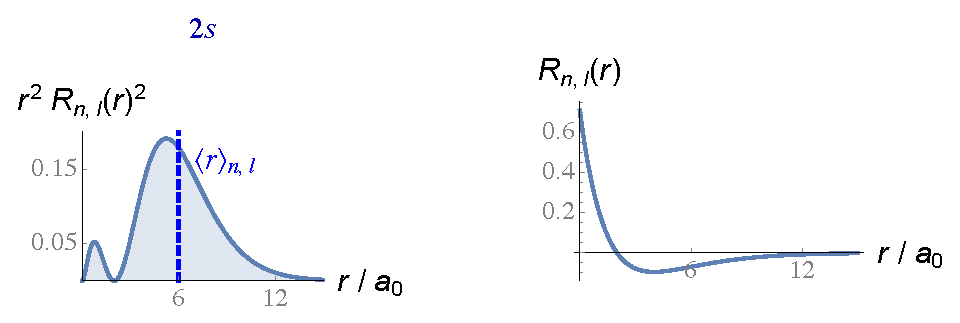
\includegraphics[scale=1]{Imagenes/Plot_Funcion_Radial_20.eps}
\end{figure}

\end{document}